\documentclass[a4paper,11pt]{article}
\usepackage[utf8]{inputenc}
\usepackage[T1]{fontenc}
\usepackage{graphicx}
\usepackage{amsmath}
\usepackage{enumerate}
\usepackage{array}
\usepackage{xcolor}
\usepackage{caption}


\begin{document}

\title{\LARGE Force-balance in FiberSim}
\date{}
\maketitle
\thispagestyle{empty}
\pagestyle{empty}

\section{Compliant myofilaments}

FiberSim is a spatially-explicit model of a half-sarcomere. It describes a compliant network of protein filaments, which is detailed below. 

\begin{figure}[h!]
\begin{center}
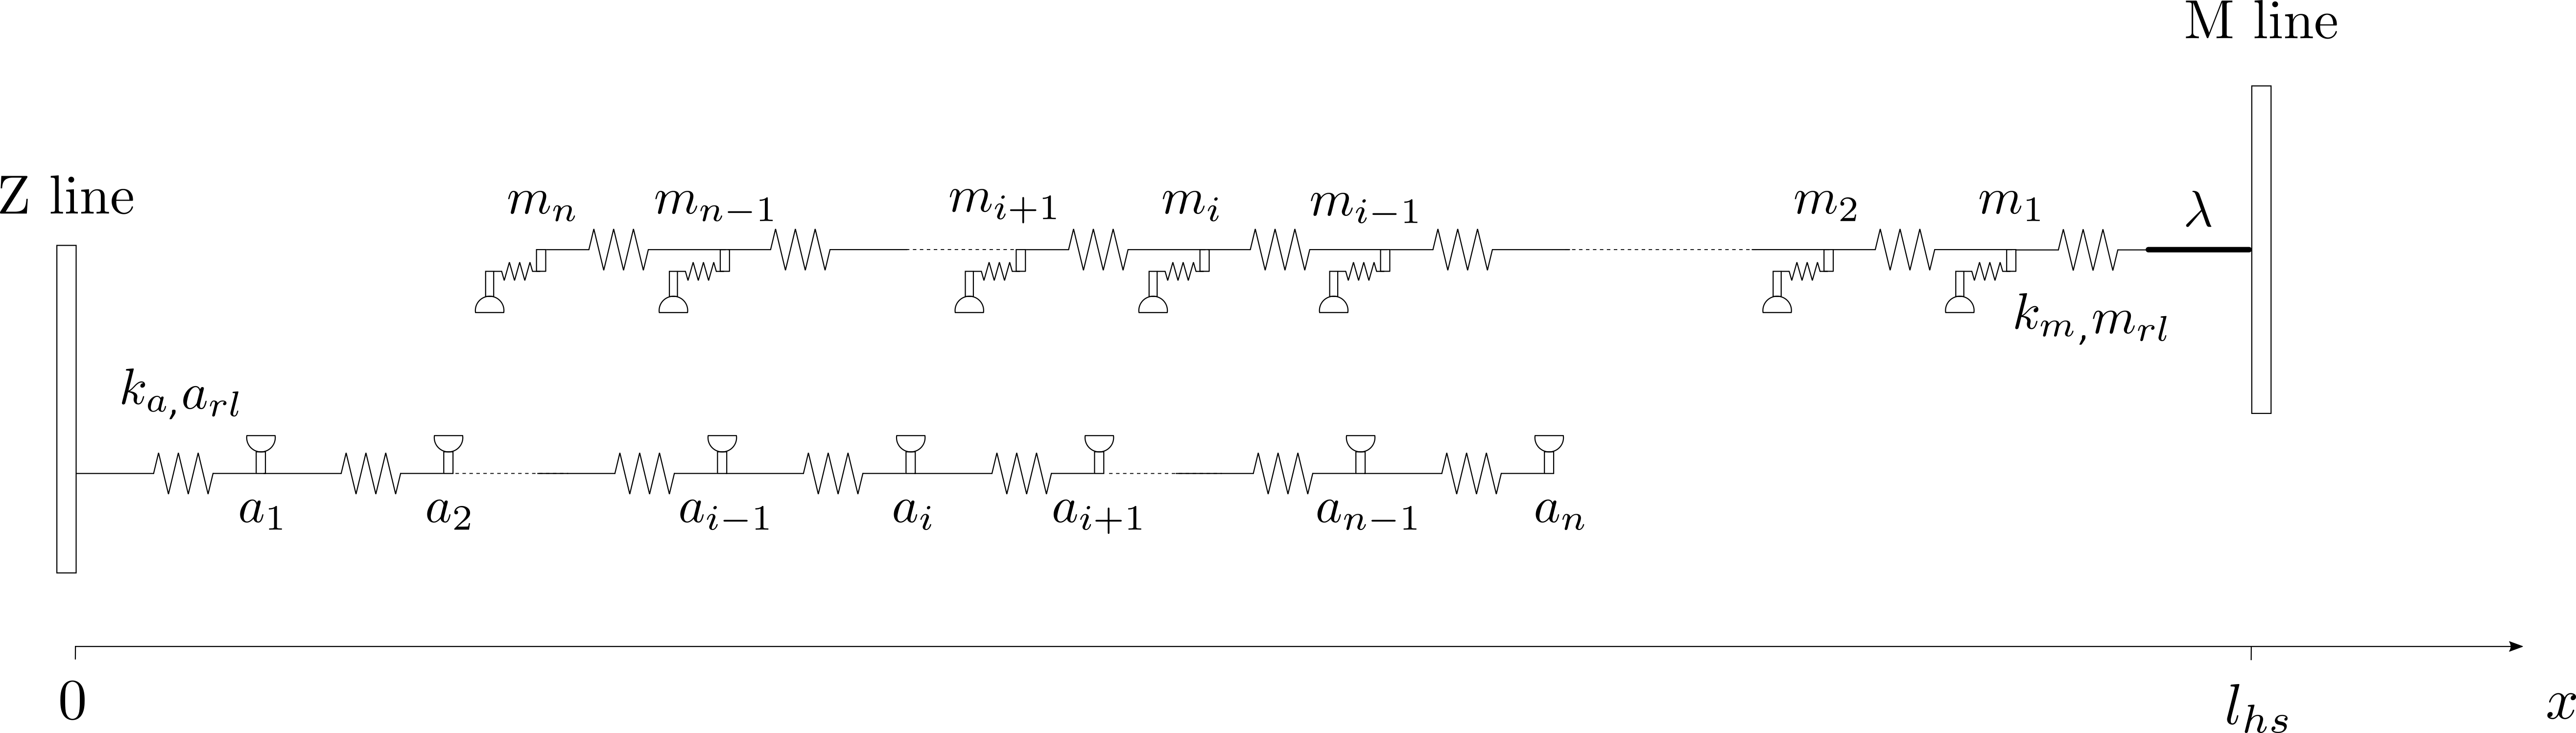
\includegraphics[width=15cm]{Pictures/Filaments.png}
\captionsetup{labelformat=empty}
\caption{Geometry and mechanical arrangement of the thick and thin filament in FiberSim.}
\end{center}
\end{figure}

\subsection{Actin filaments}

Thin filaments are composed of nodes joined by linear springs of stiffness $k_{a}$ with a resting length $a_{rl}$. If the position of the $i^{th}$ node along an x-axis is noted $a_i$, then the force-balance equations for the thin filament can be written as:

\begin{eqnarray}
\begin{aligned}
2 \, k_a \, a_1 - k_a \, a_2 &= 0 \\
-  k_a \, a_{i-1} + 2 \, k_a \, a_i - k_a \, a_{i+1} &= 0 \,\,\, (\mathrm{for} \,\, 1 < i < n) \\
-k_a \, a_{n-1} + k_a \, a_n &= k_a \, a_{rl} 
\label{thin}
\end{aligned}
\end{eqnarray}

\subsection{Myosin filaments}

Thick filaments are composed of nodes joined by linear springs of stiffness $k_{m}$ with a resting length $m_{rl}$. A rigid link of length $\lambda$ connects the thick filament to the M-line. If the position of the $i^{th}$ node along an x-axis is noted $m_i$, and the half-sarcomere length is noted $l_{hs}$, then the force-balance equations for the thick filament can be written as:


\begin{eqnarray}
\begin{aligned}
2 \, k_m \, m_1 - k_m \, m_2 &= k_m \, (l_{hs}- \lambda) \\
-  k_m \, m_{i-1} + 2 \, k_m \, m_i - k_m \, m_{i+1} &= 0 \,\,\, (\mathrm{for} \,\, 1 < i < n) \\
k_m \, m_{n-1} - k_m \, m_n &= k_m \, m_{rl}
\label{thick}
\end{aligned}
\end{eqnarray}

The system of equations \eqref{thin}-\eqref{thick} can be written in matrix form:

\begin{eqnarray}
K x = F
\label{matrix}
\end{eqnarray}

\noindent where $K$ is a matrix containing the springs stiffness, $x$ is a vector containing the positions of the actin and myosin nodes ($a_i$ and $m_i$, respectively) and F is a vector containing the constant terms (independent of nodes positions). $K$ is a tridiagonal matrix: 

\begin{eqnarray*}
K = \left [ \begin{matrix}
\# & \# & & 0 \\
\# & \ddots & \ddots &  \\
& \ddots & \ddots &  \# \\
0 &  & \# & \#  
\end{matrix}  
\right]
\end{eqnarray*} 

\noindent and numerical methods exist to solve Eq.\eqref{matrix} for $x$.

\null 

\noindent Crossbridges can bind during contraction, and thus induce crossbridge links between actin and myosin filaments. This will bring new force contributions to Eqs.\eqref{thin}-\eqref{thick}, and "non-tridiagonal" elements inside $K$. This is described in the next section.


\section{Crossbridge links}

Myosin heads located at the thick filament nodes can attach to neighboring binding sites at the thin filament nodes, thus affecting the filament lattice framework. 


\begin{figure}
\begin{center}
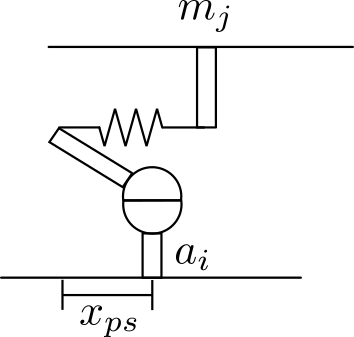
\includegraphics[scale=0.6]{Pictures/cb_link.png}
\caption{Schematic representation of a crossbridge link.}
\end{center}
\end{figure}


\noindent A crossbridge located at the $j^{th}$ thick filament node which attaches to the $i^{th}$ node of the thin filament generates a force $f_{cb}$ given by:

\begin{eqnarray}
f_{cb} = k_{cb} \, (m_j - a_i + x_{ps})
\label{matrix_cb}
\end{eqnarray}

\noindent where  $k_{cb}$ is the crossbridge spring stiffness and $x_{ps}$ is the crossbridge extension when deploying the power stroke.

\noindent This additional force on the filaments should be added to the force-balance equations \eqref{thin}-\eqref{thick}:


\begin{eqnarray}
-  k_a \, a_{i-1} + 2 \, k_a \, a_i - k_a \, a_{i+1} \, \color{red}{- \, k_{cb} \, a_i + k_{cb} \, m_j} &= \color{blue}{f_{cb} \, x_{ps}} \\
-  k_m \, m_{j-1} + 2 \, k_m \, m_j - k_m \, m_{j+1} \, \color{red}{+ \, k_{cb} \, a_i - k_{cb} \, m_j} &= \color{blue}{-f_{cb} \, x_{ps}} 
\label{thin_cb}
\end{eqnarray}

\noindent The terms in red will add non-tridiagonal, opposite elements to the $K$ matrix:

\begin{eqnarray*}
K = \left [ \begin{matrix}
\# & \# & \color{red}{\#} & 0 \\
\# & \ddots & \ddots &  \\
\color{red}{-\#} & \ddots & \ddots &  \# \\
0 &  & \# & \#  
\end{matrix}  
\right]
\end{eqnarray*} 


\noindent while the blue terms will contribute to the $F$ vector. 

\noindent Crossbridge linking toughen the numerical solving of Eq.\eqref{matrix}, which notably requires an iterative procedure to find a solution $x$ that satisfies a certain precision. 


\section{Titin}

Titin is responsible for the passive force developing within the half-sarcomere when it is streched, and for the recoil force when it is shortened. In the model, it is assumed that titin is a linear spring of stiffness $k_t$ and rest length $t_{rl}$. This spring is attached at both ends, on a particular thick and thin filament node respectively. Similar to crossbridge links, titin adds some force contribution $f_{t}$ to Eqs.\eqref{thin}-\eqref{thick}:

\begin{eqnarray}
f_{t} = k_{t} \, (m_l - a_k + t_{rl})
\label{titin}
\end{eqnarray}

\begin{figure}
\begin{center}
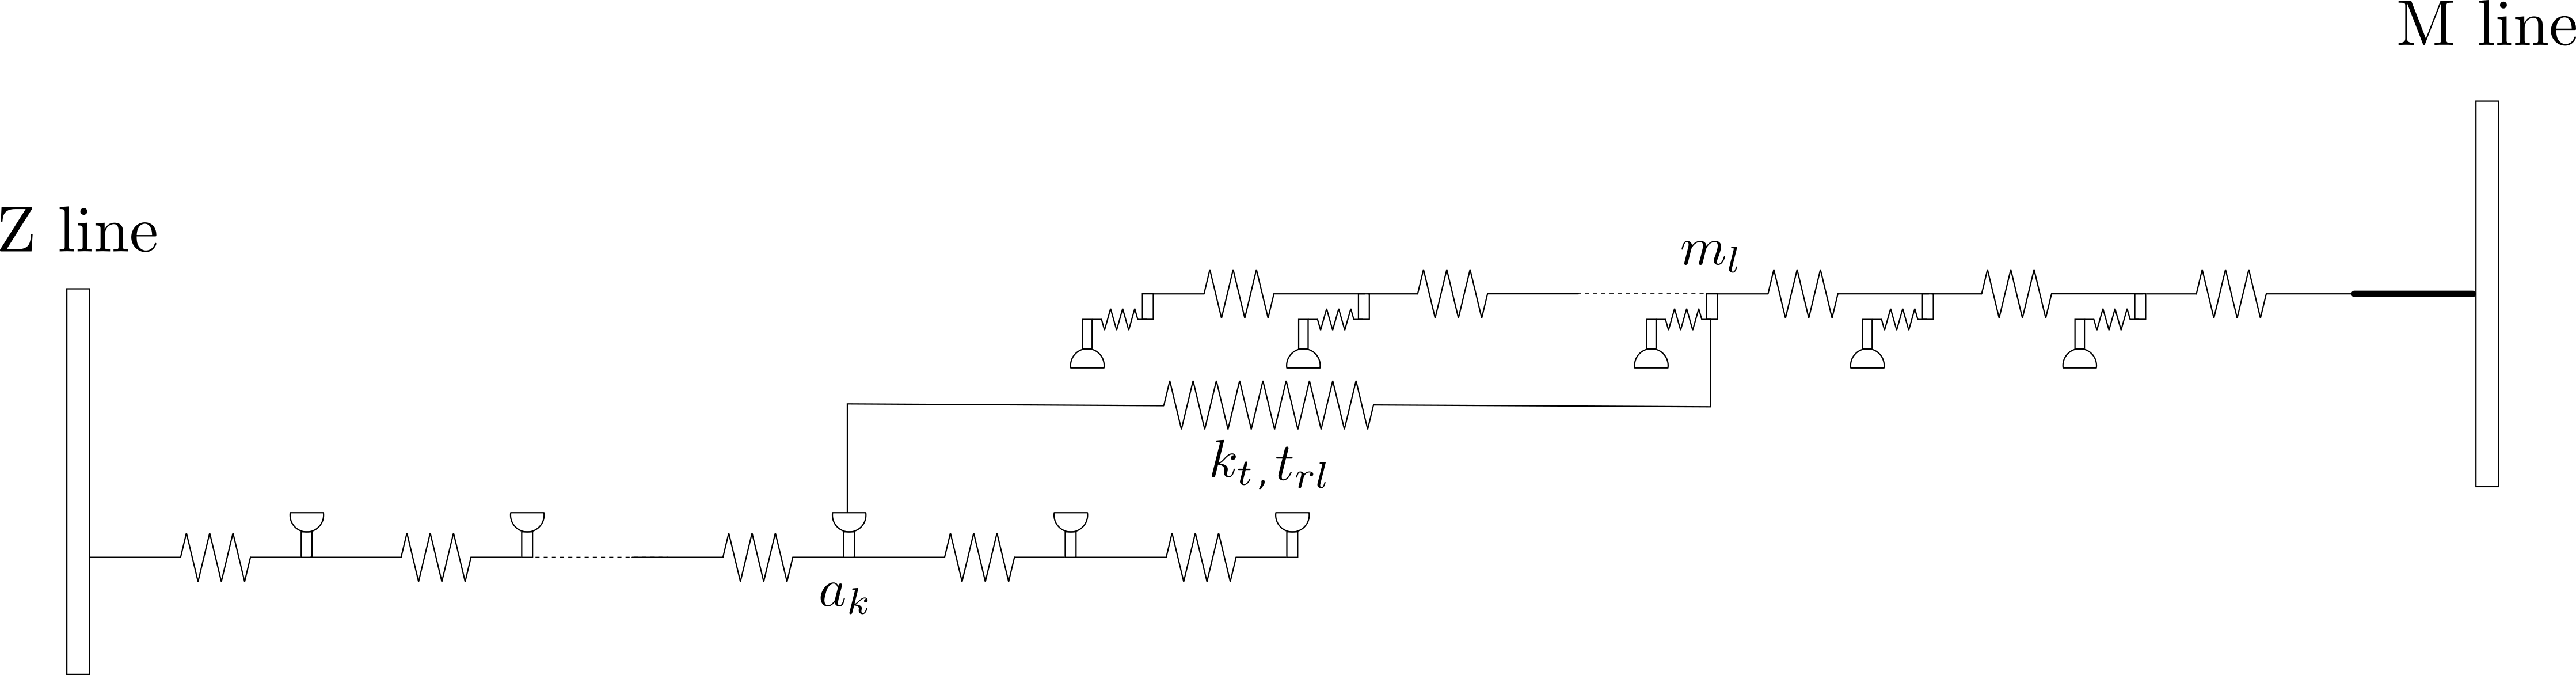
\includegraphics[width=16cm]{Pictures/titin.png}
\end{center}
\end{figure}

\section{Myosin-binding Protein C}


\end{document}


